\subsection{Method for Modeling BitTorrent Traffic Flow and Revenue of ISPs}\label{sec:p2p:methodology}

In this section we describe the methodology to estimate transit costs of ASs. First, we show where we obtain the AS affiliation of peers. Second, we explain how AS paths are inferred from AS relations and how to classify the ASs. Further on we describe different BitTorrent peer selection strategies determining the connection among peers in the Internet. Finally we introduce our transit cost model.
%\add{The methodology applied in this paper is illustrated in Fig.xyz.}

\subsubsection{AS Affiliation of Peers}

In order to know where peers are located and where BitTorrent swarms generate costs for ISPs, we need to know how the swarms are distributed over the Internet and in which ASs the peers are located. For that purpose, we use the dataset of BitTorrent movie torrents ``\texttt{Mov.}'' provided by the authors of \cite{Hossfeld2011}. A snapshot of all available movie torrents on Mininova.org was taken. The swarm sizes and peer distributions were recorded by distributed measurements. The data set consists of files with AS number and number of peers pairs for each BitTorrent swarm. Hence, they provide information for each swarm on how many peers are located in which AS. The measurement took part in April 2009 and recorded \np{126050} swarms. Peers of \np{8492} ASs are present in the swarms.


% \caption{BitTorrent swarms.} \label{tab:swarms}
% \vspace{-0.6cm}
% \begin{center}
% \begin{tabular}{|l|l|l|l|l|} \hline
% \textbf{dataset} & \textbf{type of content} & \textbf{\#torrents} & \textbf{\#ASs} & \textbf{meas. date} \\ \hline
% \textbf{mov} & movies & 126050 & 8492 & Apr. 2009 \\ \hline
% \end{tabular}
% \end{center}

% \begin{table}[ht]
% \caption{BitTorrent swarms.} \label{tab:swarms}
% \vspace{-0.6cm}
% \begin{center}
% \begin{tabular}{|l|l|l|l|l|} \hline
% \textbf{dataset} & \textbf{type of content} & \textbf{\#torrents} & \textbf{\#ASs} & \textbf{meas. date} \\ \hline
% \textbf{mov} & movies & 126050 & 8492 & Apr. 2009 \\ \hline
% \end{tabular}
% \end{center}
% \end{table}

% \begin{table}[ht]
% \caption{Classification of autonomous systems.} \label{tab:ASclass}
% \vspace{-0.6cm}
% \begin{center}
% {\footnotesize
% 	\begin{tabular}{|l|l|l|} \hline
% 		\textbf{Type} & \textbf{Classification} & \textbf{\#ASs} \\ \hline
% 		\textbf{\Tier} & AS has no providers & 11 \\ \hline
% 		\textbf{Large ISP} & AS customer tree $\geq50$ & 337 \\ \hline
% 		\textbf{Small ISP} & AS customer tree $<50$ and $\geq5$ & 1770 \\ \hline
% 		\textbf{Stub} & AS customer tree $<5$ & 36289 \\ \hline
% 	\end{tabular}
% }
% \end{center}
% \end{table}

\subsubsection{AS Relations, Paths and Classification}

To be able to estimate the transit costs produced by peers exchanging data in BitTorrent swarms, we need to know the AS paths that connect the peers. Datasets with complete AS paths would be very large and are not available to our knowledge. Hence, we infer AS paths from AS relationships.
We use the AS relationship dataset from Caida.org \cite{caidaas}. The dataset contains AS links annotated with AS relations. Each file contains a full AS graph derived from RouteViews BGP table snapshots. For our estimations we use the dataset from January 2011. The dataset consists of transit and peering relations.
% However, sibling-to-sibling is only considered by Caida and does not occur in the dataset.
% The approach that is most widely used to infer AS relationships is analyzing BGP routing tables. The data set used in this work is also produced by inferring BGP tables as described in \cite{dimitropoulos2007relationships}.
% Therefore, AS links are extracted from RouteViews BGP tables.
% RouteViews is a project that obtains information about the global routing system from the perspectives of several different backbones and locations around the Internet.
%First sibling-to-sibling links are identified by looking up organizations that own multiple AS numbers.
%Customer-to-provider relationships are inferred by a heuristic that is based on the idea of relaxing the requirement for a maximal number of valid paths and using the AS degree information to detect paths that are invalid.
%Most challenging is the inference of peer-to-peer links since paths remain valid if peer-to-peer links are replaced by a customer-to-provider or provider-to-customer link.
% The authors of \cite{dimitropoulos2007relationships} develop a heuristic which combines the strengths of previous approaches by \cite{gao2001} and \cite{di2003computing}. The inferred relationships were validated by surveys, showing that \unit[96.5]{\%} transit links and \unit[82.8]{\%} peering links of the inferred relationships are correct.


We implement the algorithm described in \cite{yang2009efficient} in Java to infer the AS paths between any two peers based on the AS relationship dataset. The authors developed a breadth first search algorithm which infers shortest paths conforming to the AS path constraints. The algorithm has runtime $O(N\cdot M)$ for finding all pair valid shortest AS paths of the graph, where $N$ is the number of AS relations and $M$ is the number of ASs.
The algorithm's input parameter is the source AS $\alpha$. For every destination AS $\beta$ the algorithm returns a set of paths $\mathbb{P}(\alpha,\beta)$, which connect $\alpha$ and $\beta$.

\begin{table}[tb]
\caption{Classification of autonomous systems.} \label{tab:ASclass}
\begin{center}
{\footnotesize
	\begin{tabular}{|l|l|l|} \hline
		\textbf{Type} & \textbf{Classification} & \textbf{\#ASs} \\ \hline
		\textbf{\Tier} & AS has no providers & 11 \\ \hline
		\textbf{Large ISP} & AS customer tree $\geq50$ & 337 \\ \hline
		\textbf{Small ISP} & AS customer tree $<50$ and $\geq5$ & 1770 \\ \hline
		\textbf{Stub} & AS customer tree $<5$ & 36289 \\ \hline
	\end{tabular}
}
\end{center}
\end{table}

Further on, we want to obtain results dependent on the AS size and type of business. Therefore we classify the ASs into \textit{stub}, \textit{small ISP}, \textit{large ISP} and \textit{tier--1}. For that purpose, we use a dataset from \cite{irlas}, which provides information about the number of customers and providers for each AS number. This dataset is from November 2011 and is used to classify the ASs according to the size of their customer tree.
\reftab{tab:ASclass} lists the different AS types and their classification. \Tier ASs are the largest ASs building the core of the Internet. \Tier ASs do not have providers. In their dataset 11 \tier ASs are identified. If an AS has a customer tree that contains at least 50 nodes, it is classified as a large ISP. An AS is classified as small ISP if its customer tree has less than 50 but at least 5 nodes. Most ASs are stub ASs, which have a customer tree that is smaller than 5.

\subsubsection{BitTorrent Neighbor Set Creation}

The BitTorrent neighbor set of a peer defines the data exchange with other peers in BitTorrent swarms. Neighbors are the peers in the swarm which are connected to a peer. It has to be noted that the measurements in \cite{Hossfeld2011} do not reveal the real composition of the neighbor sets of the swarms. Further on, neighbor sets are randomly generated and differ for every peer, which makes them hard to capture. Hence, we estimate the composition of the neighbor sets in three simple ways, \textit{random}, \textit{locality} and \textit{selfish-ISP}.
The number of peers in the swarm is the swarm size $S$. The number of neighbors is denoted as $N$ with $N\leq S-1$. In the standard BitTorrent implementation a client can connect to up to 40 peers, so we set the maximum size of the neighbor set to $N_{max}=40$. Hence, the neighbor set for each peer in a swarm with size $S$ has size
\begin{equation}
N=min(N_{max},S-1) \, .
\end{equation}
We add peers to the neighbor set until it contains $N$ neighbors according to the following algorithms.
\paragraph{a) random}
In the random selection strategy we add random $N$ peers of the swarm to the neighbor set. In the standard BitTorrent algorithm the selection of neighbors is also random. Hence, with this selection strategy we try to estimate the traffic and costs produced by the standard BitTorrent algorithm.
\paragraph{b) locality}
In the locality algorithm we sort the AS paths connecting two peers by the number of AS hops. Then we add the peers according to the sorted set of increasing AS paths until $N$ peers are in the neighbor set. Note that first the peers located in the same AS, i.e., zero AS hops, are added. This selection algorithm is used to optimize the swarm by minimizing AS hops between peers and thereby potentially reducing latencies. Hence, the motivation for this algorithm is to optimize the swarm from the overlay's point of view.
In practice, such a selection could be realized e.g. with an \emph{iTracker} \cite{Xie2008}, a database which maps IP-addresses to autonomous system numbers, or other ALTO mechanisms.
\paragraph{c) selfish-ISP}
The selfish-ISP selection algorithm tries to select as many peers from customer ASs as possible. Until the neighbor set contains $N$ peers it first adds peers from paths starting with provider-to-customer links, then peers of the same AS, then paths starting with peering links and finally customer-to-provider links.
This selection algorithm is used to maximize the revenue of ISPs. This is achieved by the selfish-ISP strategy by selecting preferentially peers that are connected by customers and avoiding peers at providers. In practice an ISP must be able to control the neighbor set. Hence, ALTO mechanisms for selfish-ISP selection must be controllable by the ISP. One approach is that the ISP provides an information service to guide the peer selection, such as an oracle \cite{Aggarwal2007} or an information service \cite{hossfia}.

% \begin{figure*}[bt]
% \begin{minipage}[b]{0.49\textwidth}
% 	\centering
% 	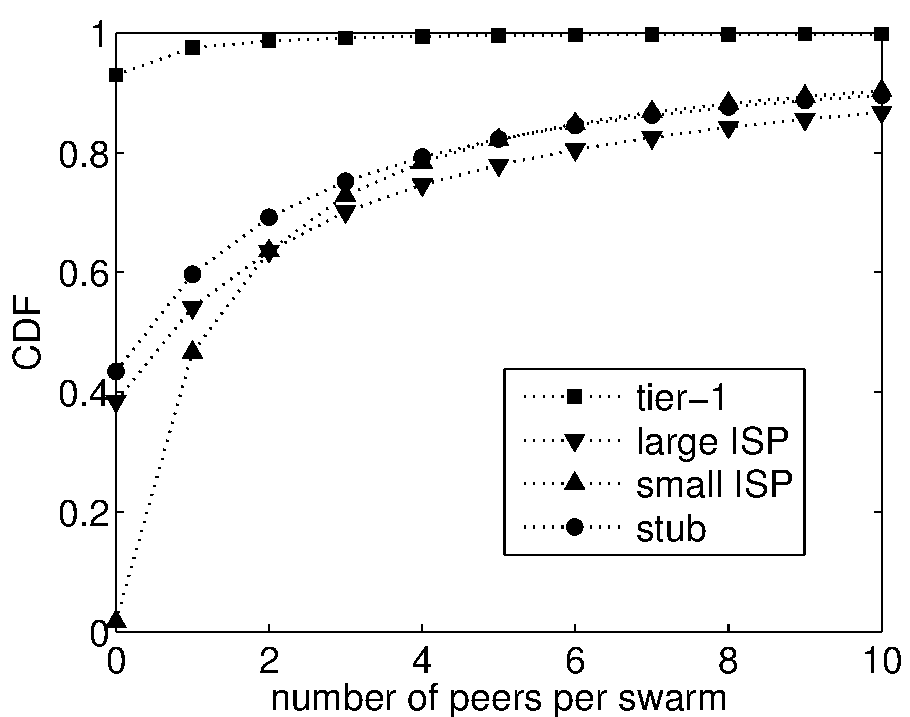
\includegraphics[width=\textwidth]{aslevel/p2p/methodology/figs/CDF_npeers_perswarm}
%  	\caption{CDF of the number of peers per swarm depending on the different ISP classes.}
%  	\label{fig:CDF_npeers_perswarm}
% \end{minipage}
% \hspace{0.01\textwidth}
% \begin{minipage}[b]{0.49\textwidth}
% 	\centering
% 	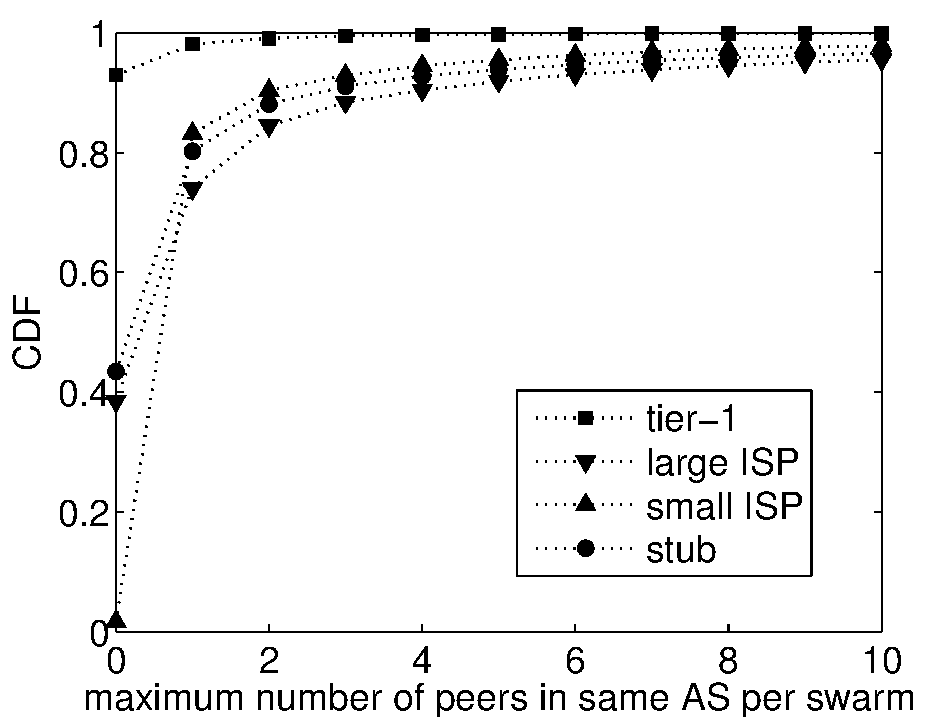
\includegraphics[width=\textwidth]{aslevel/p2p/methodology/figs/CDF_maxpeers_perswarm_perAS}
%  	\caption{CDF of the maximum number of peers in same AS per swarm depending on the tier.}
%  	\label{fig:CDF_maxpeers_perswarm_perAS}
% \end{minipage}
% \end{figure*}

%\begin{figure*}[bt]
%\begin{minipage}[b]{0.32\textwidth}
%	\centering
%	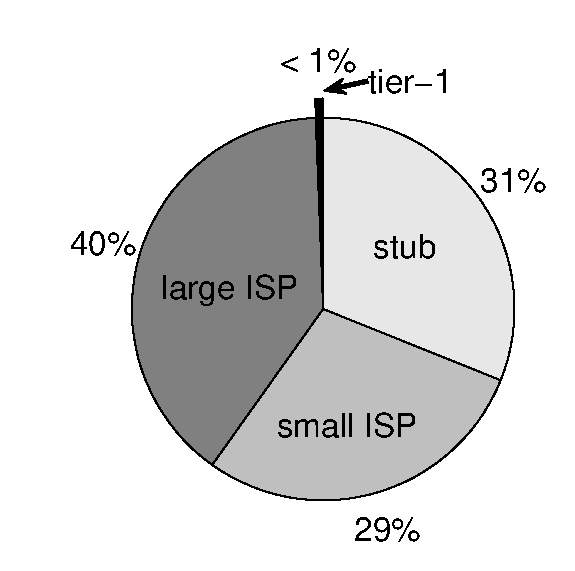
\includegraphics[width=0.8\textwidth]{aslevel/p2p/methodology/figs/npeers_perTier}
% 	\caption{Ratio of peers per ISP class aggregated over all swarms in the measurement set.}
% 	\label{fig:npeers_perTier}
%\end{minipage}
%\hspace{0.01\textwidth}
%\begin{minipage}[b]{0.32\textwidth}
%	\centering
%	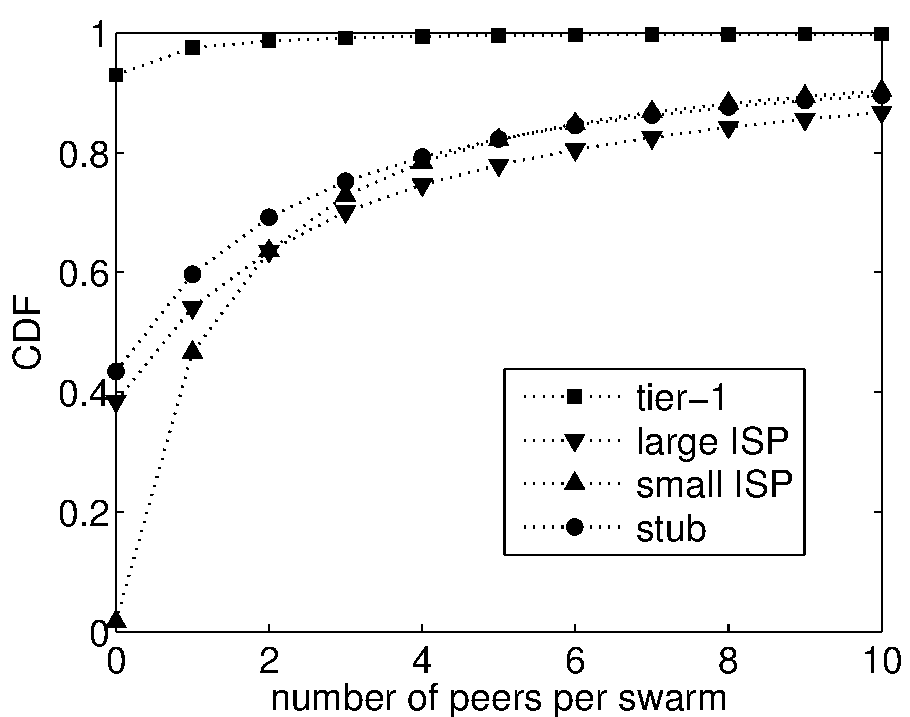
\includegraphics[width=\textwidth]{aslevel/p2p/methodology/figs/CDF_npeers_perswarm}
% 	\caption{CDF of the number of peers per swarm depending on the different ISP classes.}
% 	\label{fig:CDF_npeers_perswarm}
%\end{minipage}
%\hspace{0.01\textwidth}
%\begin{minipage}[b]{0.32\textwidth}
%	\centering
%	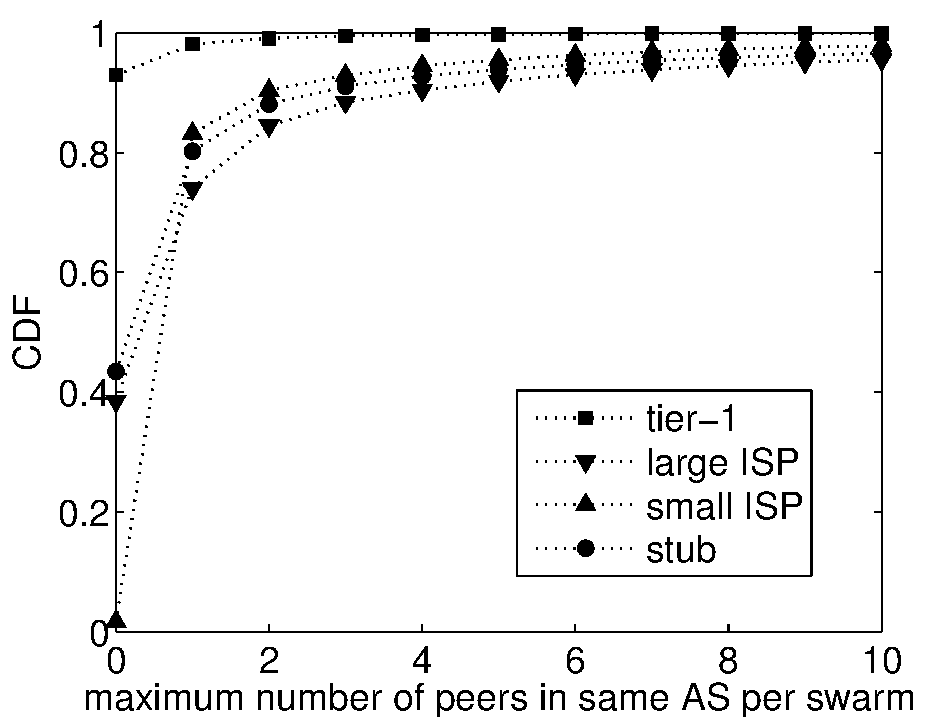
\includegraphics[width=\textwidth]{aslevel/p2p/methodology/figs/CDF_maxpeers_perswarm_perAS}
% 	\caption{CDF of the maximum number of peers in same AS per swarm depending on the tier.}
% 	\label{fig:CDF_maxpeers_perswarm_perAS}
%\end{minipage}
%\end{figure*}

\subsubsection{Cost Model}

To be able to estimate the costs for ASs arising from transit services, we need to know how much traffic is generated and how much providers charge customers for forwarding the traffic.
We consider a snapshot and assume instantaneous traffic rates, i.e., the file-size of the download can be neglected.
For simplicity we make assumptions on how much traffic is generated in each swarm, depending on the the number and location of peers.
\newtheorem{assa}{Assumption}\begin{assa}\label{npeers}
The traffic generated by a peer is equally shared among its neighbors.
\end{assa}
\newtheorem{assb}[assa]{Assumption}\begin{assb}\label{ntraffic}
All peers generate traffic at the same rate.
\end{assb}
\newtheorem{assc}[assa]{Assumption}\begin{assc}\label{npaths}
The traffic between ASs is equally shared among the paths that connect them.
\end{assc}
In practice, traffic rates are allocated by BitTorrent's choke algorithm, which takes into account the upload and download speed of the other peers. Further on, traffic is generally not shared among different AS paths. But, since we consider the aggregated traffic of a large number of swarms, we argue that these assumptions are reasonable and the results do not change significantly.
%and differ for every peer according to its upload bandwidth. Further on,
\paragraph{Traffic Amount}
% We distinguish inter AS traffic and intra AS traffic. Intra-AS traffic is the traffic locally generated by peers which are in the same AS. For intra-AS traffic the AS path has zero AS hops. We estimate the amount of intra-AS traffic proportional to the number of possible directed connections between peers in the source AS. Let $n_{src}$ be the number of peers in the source AS and $\hat n_{src}$ be the number of peers that are in the source AS and in the neighbor set. Then the intra-AS traffic is calculated by
% \begin{equation}
% \frac {\hat n_{\alpha} \cdot (\hat n_{\alpha}-1)} {N} .
% \end{equation}

We use the above assumptions to estimate the traffic generated by the BitTorrent swarms.
Assumption~\ref{npeers} implies that the traffic sent by a given peer $p_1$ is equally distributed among its $N$ neighbors. Hence, the traffic $p_1$ sends to a neighbor $p_2$ is
\begin{equation}
T(p_1,p_2)=\frac 1 N \, .
\end{equation}
Assumption~\ref{ntraffic} implies that the traffic originating in a given AS $\alpha$ is proportional to the number of peers located in this AS.
Let $\mathcal S$ be the set of all swarms, then the traffic of all swarms that is sent from AS $\alpha$ to AS $\beta$ can be calculated by
\begin{equation}
T(\alpha,\beta)=\sum_{s \in \mathcal S}\sum_{\genfrac{}{}{0pt}{}{\alpha\in s,}{p_1\in\alpha}}\sum_{\genfrac{}{}{0pt}{}{\beta\in s,}{p_2\in\beta}}T(p_1,p_2) \, .
\end{equation}

%Since the traffic is equally distributed among the neighbors, the inter-AS traffic originating from a source AS $src$ is proportional to the number of neighbors $\hat n_{dst}$ in the destination AS $dst$.
The set of AS paths connecting AS $\alpha$ with $\beta$ obtained by the AS inference algorithm is given by $\mathbb P(\alpha,\beta)$.
Assumption~\ref{npaths} implies that the traffic between $\alpha$ and $\beta$ and later the costs are shared equally among the paths in $\mathbb P(\alpha,\beta)$. Hence, we can calculate the traffic on a path $P\in\mathbb P(\alpha,\beta)$.

\begin{equation}
T(P)=\frac 1 {|\mathbb P(\alpha,\beta)|} \cdot T(\alpha,\beta),\;\;\; P\in\mathbb P(\alpha,\beta) \, .
\end{equation}

Next we can calculate the link load $L(\alpha,\beta)$ on the link between two directly connected ASs $\alpha$ and $\beta$. We use $\alpha\leftrightarrow \beta \in P$ as notation for a direct link between $\alpha$ and $\beta$ on the path $P$. The link load is the sum of the load on all paths sharing the link $\alpha\leftrightarrow\beta$.

\begin{equation}\label{equ:linkload}
L(\alpha,\beta)=\sum_{P|\alpha\leftrightarrow \beta \in P} T(P) \, .
\end{equation}

As we consider each AS in a swarm as source AS, the outgoing AS traffic equals the incoming AS traffic. Therefore, we only consider the outgoing AS traffic as inter-AS traffic. The in- and outgoing traffic for AS $\alpha$ is the sum of all loads on links connecting $\alpha$.

\begin{equation}\label{equ:outgoing}
in(\alpha) = out(\alpha) = \sum_{\beta| \exists P, \alpha\leftrightarrow \beta \in P} L(\alpha,\beta) \, .
\end{equation}

In the following we estimate the transit costs. The transit costs are weighted by the link loads defined in this section.
% Hence, we estimate the outgoing traffic $\zeta(p)$ of ASs on paths $p \in \Gamma_{src,dst},$ for $n_{src}$ peers in $src$, and $\hat n_{dst}$ out of $N$ neighbors in $dst$ by

% \begin{equation}
% \zeta(p) = \frac {n_{src} \cdot \hat n_{dst}} {N\cdot |\Gamma_{src,dst}|} .
% \end{equation}

% Hence, in each swarm a total traffic of
% \begin{equation}
% \sum_{src \in \Lambda} \sum_{dst \in \Lambda \backslash \{src\}} \left(\frac {n_{src} \cdot n_{dst}} {N\cdot |\Gamma_{src,dst}|} + \frac {n_{src} \cdot (n_{src}-1)} {N}\right)
% \end{equation}
% is produced. With the set of ASs $\Lambda$.

\subsubsection{Transit Costs}

The business relationships between ISPs define the exact transit costs, but they are part of the private contracts between the ISPs. Hence, we develop a simple model for the arising transit costs. It is common that peering ASs exchange their traffic and the traffic of their customers without charging. Hence, we assume no costs for peering links. The amount a customer pays a provider for transit for a specific volume of traffic is unclear, so we set it to one cost unit, i.e., $1$. That is not the case in practice, but as we have a large number of ASs and swarms, we get a qualitatively good estimation.\\
%For given $\alpha$ and $\beta$ and the set of AS paths $\Gamma_{src,dst}$ we estimate costs, revenues and the balance for every AS occurring on the AS paths connection $src$ and $dst$.
The \textit{costs} of an AS $\alpha$ are increased, if it acts as customer of an AS $\beta$. The costs are increased by one unit weighted by the amount of traffic on the link connecting $\alpha$ and $\beta$, i.e., $L(\alpha, \beta)$ from \refequ{equ:linkload}. Let $\mathcal P(\alpha)$ be the set of providers of $\alpha$, and let $\mathcal C(\alpha)$ be the set of customers of $\alpha$. Then we can calculate the costs of AS $\alpha$ emerging in all swarms as follows.
\begin{equation}\label{equ:costs}
costs(\alpha) = \sum_{\beta\in\mathcal P(\alpha)} L(\alpha,\beta) \, .
\end{equation}
In the same way we can calculate the \textit{revenues} for all AS links and swarms, where $\alpha$ acts as provider.
\begin{equation}\label{equ:revenues}
revenues(\alpha) = \sum_{\beta\in \mathcal C(\alpha)} L(\alpha,\beta) \, .
\end{equation}
The \textit{balance} is the difference between revenues and costs.
\begin{equation}\label{equ:balance}
balance(\alpha) = revenues(\alpha)-costs(\alpha) \, .
\end{equation}
